\chapter{Self-organizing Feature Maps}
Neurons in layers excite its closest neighbours via \emph{lateral connections} and inhibit the distance neighbours. \emph{Lateral} interactions create \emph{competition and cooperation} among them. 

\section{Self-Organizing Neural Networks}
\begin{figure}[!h]
\centering
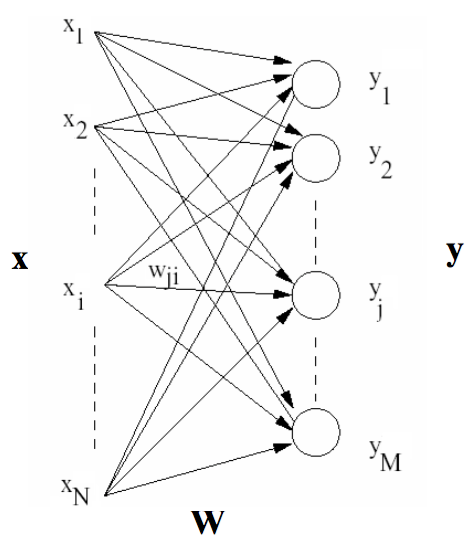
\includegraphics[width=8cm]{chapter9_1}
\end{figure}

\section{Similarity Measures}
Euclidean distance:
\begin{equation*}
\begin{split}
distance &= \|\boldsymbol{x}_i - \boldsymbol{x}_j \| \\
&= \sqrt{(\boldsymbol{x}_i - \boldsymbol{x}_j)^{T} (\boldsymbol{x}_i - \boldsymbol{x}_j)} \\
&= \sqrt{\sum_k (x_{ik} - x_{jk})^{2}}
\end{split}
\end{equation*}
Cosine similarity:
$$\cos \theta = \frac{\boldsymbol{x}_i^{T} \boldsymbol{x}_j}{\|\boldsymbol{x_i}\|\|\boldsymbol{x_j}\|}$$

\section{Kohonen's Neural Network}
Synaptic input to the output layer:
$$\mathbf{u = Wx}$$
The ouput of the network:
$$\mathbf{y = f(u)}$$

\subsection{Winner-Takes-All Rule}
If winner is the $m$ th neuron, then:
$$m = \arg\!\max_{i=1...M} u_i$$
The output of the neuron:
$$y_m = 1$$
The output of other neurons:
$$y_i = 0$$

\subsection{Kohonen Learning Rule}
Prior to learning, all the weight vectors are randomly initialized and then normalized:
$$\mathbf{\hat{w}} = \frac{\mathbf{w}_j}{\|\mathbf{w}_j\|}$$
Next, \emph{find the winner} and update its weight:
\begin{equation*}
\begin{split}
\mathbf{w}_m^{t+1} &= \mathbf{\hat{w}}_m^{t} + \Delta \mathbf{\hat{w}}_m^{t} \\
&= \mathbf{\hat{w}}_m^{t} + \alpha^{t}(\mathbf{x} - \mathbf{\hat{w}}_m^{t})
\end{split}
\end{equation*}
The new weight is then normalized.

\subsubsection{Neurons with the highest synaptic inputs are winner}
We want to find the closest weight vector $w$ to current input $x$:
$$\| \mathbf{x} - \mathbf{\hat{w}}_m \| = \!\min_{j=1...M} \| \mathbf{x} - \mathbf{\hat{w}}_j \|$$
\begin{equation*}
\begin{split}
\| \mathbf{x} - \mathbf{\hat{w}}_m \| &= \Big[(\mathbf{x} - \mathbf{\hat{w}}_m)^{T}(\mathbf{x} - \mathbf{\hat{w}}_m) \Big]^{\frac{1}{2}} \\
&= \Big(\mathbf{x^{T}x - 2\hat{w}_{m}x + 1} \Big)^{\frac{1}{2}}
\end{split}
\end{equation*}
Searching for the closest weight vector is equivalent to:
\begin{equation*}
\begin{split}
\mathbf{\hat{w}}_m^{T} \mathbf{x} &= \!\max_{j=1...M} \mathbf{\hat{w}}_j^{T} \mathbf{x} \\
u_m &= \!\max_{j=1...M} u_j
\end{split}
\end{equation*}

\subsubsection{Impact of the Learning Rule}
Kohonen learning rule should increase the chances of winning of neuron $m$ after each iteration. It means that:
$$u_m^{new} > u_m^{old}$$
Proof:
$$u_m^{new} - u_m^{old} = \alpha (\| x \|^{2} - \| \hat{w}_m^{T} \| \|x\|\cos \theta)$$
But $\cos \theta \le 1$, $1 > \alpha > 0$ and $\|\hat{w}\| = 1$, assume $\|x\| = 1$, so: 
$$u_m^{new} > u_m^{old}$$
That's why we need to normalize weight after each iterations.

\subsubsection{Geometrical Interpretation of the Learning Rule}
$\Delta \mathbf{\hat{w}}_m$ is a rotation of $\mathbf{\hat{w}}_m$ toward input vector $\mathbf{\hat{x}}$ without significant length change. 
\begin{figure}[!h]
\centering
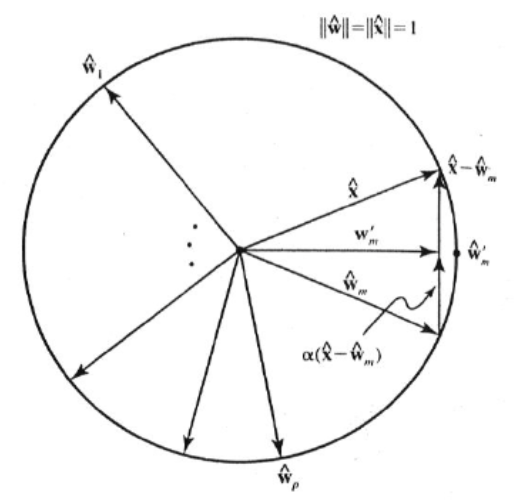
\includegraphics[width=5cm]{chapter9_2}
\end{figure}

\subsubsection{Initialization of the Weights}
Convex combination:
$$\mathbf{w}_j^{0} = \frac{1}{\sqrt{n}} (1 1 ... 1)^{T}$$

\subsubsection{Limitation of Basic Kohonen Network}
\begin{enumerate}
\item Linearly non-separable pattern cannot be efficiently handled
\item Not always successful for linearly separable patterns
\item Neurons with initial weights far from any input vector may never win
\end{enumerate}

\section{Kohonen Self-Organizing Feature Maps}
In the training phase, we update weight vector of winning neuron $m$ \emph{and its neighbours} according to the radius $N_m^{t}$. The weight of winning neuron is updated using the method described in previous section. The weight of neighbours is updated by:
$$\Delta \mathbf{w}_j^{new} = \alpha(j,t) (\mathbf{x} - \mathbf{w}_j^{old})$$
$$\forall j \in N_m(t)$$

\section{Vector Quantization}
Vector quantizer $Q$ is a mapping:
$$Q:\mathbf{R}^{n} \rightarrow C$$
\begin{center}where $C={c_1 c_2 \ldots c_M}$ is a set of vectors or codewords\end{center}
For an input vector $\mathbf{x} \in R^{n}$ the output of quantizer ca be implemented in competitive neural network
$$Q(\mathbf{x}) = c_m$$
$$if\ \|\mathbf{x-c_m} \| = \!\min_{i} \| \mathbf{x-c_i} \|$$

\subsection{LVQ1}
LVQ is a supervised form of algorithm for Vector Quantization
\begin{enumerate}
\item The weight vector $\mathbf{w_j}$ are defined using SOFM
\item For each input pattern, find winning neuron $m$
\item If the desired winner for $\mathbf{x}$ is $q$
$$
\mathbf{w}_m^{new} = 
\begin{cases}
\mathbf{w}_m + \alpha (\mathbf{x} - \mathbf{w}_m) & m = q \\
\mathbf{w}_m - \alpha (\mathbf{x} - \mathbf{w}_m) & m \ne q
\end{cases}
$$
$$w_j^{new} = w_j, \forall j \ne m$$
\end{enumerate}

\subsection{LVQ2}
Same as LVQ1, but learning is applied only if:
\begin{enumerate}
\item The desired winner is not the winner, $m \ne q$
\item The second closest prototype vector is $w_{m*}$ the correct class
\item The input vector is close to the boundary between $\mathbf{w}_m$ and $w_{m*}$
\end{enumerate}
\begin{equation*}
\begin{split}
\mathbf{w}_{m*}^{new} &= \mathbf{w}_{m*} + \alpha (\mathbf{x} - \mathbf{w}_{m*}) \\
\mathbf{w}_{m}^{new} &= \mathbf{w}_{m} + \alpha (\mathbf{x} - \mathbf{w}_{m}) \\
w_j^{new} &= w_j, \forall j \ne m, m*\end{split}
\end{equation*}
